\documentclass[a4paperm]{article}
%\documentclass[12pt,twocolumn]{article}

\usepackage[T2A]{fontenc}
\usepackage[utf8]{inputenc}
\usepackage[russian,english]{babel}
\usepackage{amsmath,amsthm,amssymb,stackrel}
\usepackage[affil-it]{authblk}
\usepackage{cite}
\usepackage{scrextend}
\usepackage{verbatim}
\usepackage{paralist}
\usepackage[mediumspace,mediumqspace,Grey,squaren]{SIunits}
\addtokomafont{labelinglabel}{\sffamily}
\usepackage{amsmath}
\usepackage{graphicx}
 \usepackage[usenames, dvipsnames]{color}
 \usepackage{multirow}
 \usepackage{longtable}
 \usepackage{lineno}
 
 \usepackage{xr}
 
 
%\usepackage[none]{hyphenat} %no nyphenation

\usepackage{SIunits}
\usepackage{miller}
\usepackage[version=3]{mhchem}

\usepackage{float} %H with figures

\setlength{\parindent}{5ex}

 \usepackage{newfloat} %For numbering of supplemmentary figures
 \DeclareFloatingEnvironment[name={Supplementary Figure}]{suppfigure}

\graphicspath{{figures/}}
\externaldocument{supplementary/mg2co4_supp}


\begin{document}

%\linenumbers

\title{The formation of Mg-orthocarbonate through the reaction MgCO$_3$ + MgO = Mg$_2$CO$_4$ at Earth's lower mantle $P$--$T$ conditions}


\author[1,2]{Pavel N. Gavryushkin
   \thanks{Electronic address: \texttt{gavryushkin@igm.nsc.ru, p.gavryushkin@g.nsu.ru}; Corresponding author}}     
\author[1,2]{Dinara N. Sagatova}
\author[1]{Nursultan Sagatov}
\author[3]{Konstantin D. Litasov}

\affil[1]{Sobolev Institute of Geology and Mineralogy, Siberian Branch of Russian Academy of Sciences, prosp. acad. Koptyuga 3, 630090 Novosibirsk, Russia}
\affil[2]{Novosibirsk State University, Pirogova 2, Novosibirsk 630090, Russia}
\affil[3]{Vereshchagin Institute for High Pressure Physics RAS, 108840, Troitsk, Moscow, Russian Federation}

\date{}
\maketitle

%\linenumbers

\begin{abstract}
Orthocarbonates of alkaline-earth metals are the newly discovered class of compounds stabilized at high pressures.
Mg-orthocarbonates are the potential carbon host phases, transferring oxidized carbon in the Earth's lower mantle up to the core-mantle boundary.
Here, we demonstrate the possibility for the formation of Mg$_2$CO$_4$ in the lower mantle at pressures above 50 GPa, by {\it ab initio} calculations.
Mg$_2$CO$_4$ is formed by the reaction MgCO$_3$ + MgO = Mg$_2$CO$_4$, proceeding only at high-temperatures.
At 50 GPa the reaction starts at 2200 K.
The temperature decreases with pressure and drops down to 1085 K at the pressure of the Earth's core-mantle boundary, near 140 GPa.
Two stable structures, Mg$_2$CO$_4$-$Pnma$ and Mg$_2$CO$_4$-$P2_1/c$, were revealed.
Mg$_2$CO$_4$-$Pnma$ is isostructural to forsterite (Mg$_2$SiO$_4$), while Mg$_2$CO$_4$-$P2_1/c$ is isostructural to larnite ($\beta$-Ca$_2$SiO$_4$).
Transition pressure from Mg$_2$CO$_4$-$Pnma$ to Mg$_2$CO$_4$-$P2_1/c$ is around 80 GPa.
Both phases are dynmaically stable on decompression up to the ambient pressure and temperature. 
This assumes the possibility for their finding in natural samples of high-pressure rocks.
Mg$_2$CO$_4$-$Pnma$ has a melting temperature more than 16\% higher  than the melting temperature of magnesite (MgCO$_3$).
At 23.7 GPa, 35.5 GPa, and 52.2 GPa, Mg$_2$CO$_4$-$Pnma$  melts at 2661 K, 2819 K, and 3109 K, respectively.
Acoustic wave velocities $Vp$ and $Vs$ of Mg$_2$CO$_4$-$Pnma$ are very similar to that of magnesite, while universal anisotropy of Mg$_2$CO$_4$-$Pnma$ is stronger than that of magnesite, as well as coefficient $A^U$ is larger for orthocarboante .



\end{abstract}


\section*{Introduction}

During the recent decade, the crystal structure prediction technique became an integral part of high-pressure research. 
Numerous experimental synthesis were guided by this technique, for instance, the synthesis of the high-pressure phases of alkaline carbonates Li$_2$CO$_3$, Na$_2$CO$_3$, and K$_2$CO$_3$ \cite{gavr2016, gavr2019_alk, grzechnik2003}  and alkaline-earth carbonates CaCO$_3$, MgCO$_3$, and CaMg(CO$_3$)$_2$ \cite{oganov2006, pickard2015, gavr2017_aragII, smith2018, solomatova2017_fedol, binck2020_dol, merlini2017_dol}.
 
Orthocarbonates are another example for experimental confirmation of theoretically predicted structures.
%The possibility for the synthesis of alkaline orthocarbonate has been suggested from the theoretical considerations \cite{alshemali2002, cancarevich2007}.
%However, these predictions are still unverified by the experiment.
The stability of the alkaline-earth orthocarbonates has not been considered till the last year.
The performed crystal structure prediction in the MgO -- CO$_2$ and CaO -- CO$_2$ systems have revealed $sp^3$-bonded structures with the intermediate stoichiometries,  Ca$_3$CO$_5$ and CaC$_2$O$_5$, stabilized at high pressures \cite{yao2018}. 
Thermodynamically stable structures of orthocarbonates with the Сa$_2$CO$_4$ or Mg$_2$CO$_4$ stoichiometry  have not been revealed in these calculations.
Assuming the stochastic nature of the used methods of crystal structure prediction and possibility that some favorable structures can be missed in the calculation, we have performed a thorough search using both evolutionary algorithms (USPEX) and {\it ab initio} random methods (AIRSS) within the stoichiometry of orthocarbonates M$_2$CO$_4$, where M is alkaline-earth metal, Mg, Ca, Sr, or Ba.
As the result of this investigation, the structure Ca$_2$CO$_4$-$Pnma$ was obtained \cite{sagatova2020_ortho}.
This structure lies above the energetic convex hull in the CaO -- CO$_2$ system, i.e. it is stable relative to the decomposition on the known phases of this system, in particular to the mixture of CaO+CaCO$_3$.
Further theoretical search has also shown that the similar structures of Sr and Ba orthocarbonates, Sr$_2$CO$_4$-$Pnma$ and Ba$_2$CO$_4$-$Pnma$, are stable at relatively low pressures \cite{gavr2020_htxrd}. 
Recent experimental synthesis combined with single-crystal X-ray diffraction method have unambigously confirmed the stability of the predicted Ca$_2$CO$_4$-$Pnma$ and Sr$_2$CO$_4$-$Pnma$ structures \cite{laniel2021_sr2co4,binck2021_ca2co4}.

Undoubtedly, the most interesting orthocarbonate for the Earth sciences is the orthocarbonate of Mg. 
This compound can be readily formed within the slab subducted in the Earth's lower mantle from the locally abundant MgCO$_3$ and MgO by the simple reaction MgCO$_3$ + MgO = Mg$_2$CO$_4$.
The formation of Mg$_2$CO$_4$ with spinel structure have been speculatively suggested by Fyfe back in 1970 \cite{fyfe1970}.
Then formation of Mg$_2$CO$_4$ have been hypothesized by Irwing AJ and Wyllie PJ \cite{irving1973}, and T. Katsura \cite{katsura1991_mgco3}.
However, as no experiments \cite{irving1973}, no calculations \cite{yao2018,sugano1980} have revealed any intermediate phases in the system MgO--MgCO$_3$, the possibility for the formation of Mg-orthocarboantes at high pressures is unclear.

In the present study, using crystal structure prediction techniques, we revealed new structures of Mg-orthocarboante, Mg$_2$CO$_4$, stable against decomposition on MgCO$_3$ and MgO, having chances to be formed at the Earth's lower mantle $P$--$T$ conditions.


%%%%%%%%%%%%%%%%%%%%%%%%%%%%%%%%%%%%%
		\section*{Methods}
%%%%%%%%%%%%%%%%%%%%%%%%%%%%%%%%%%%%%

To increase the chances for finding the energetically favorable structures we have used both USPEX and AIRSS methods, each of which has apparent advantages \cite{oganov2019}.
{\it Ab initio} structure prediction was complemented by the prediction technique based on the known structures of Mg- and Zn- orthosilicates with isolated [SiO$_4$] tetrahedrons, as well as sulfates with isolated [SO$_4$] tetrahedrons. 
Mg$_2$CO$_4$ structures were produced from these structures by the corresponding replacement of the cations and consequent local optimizations.
The following crystal structures have been used (numbers in parentheses indicate the number of formula units (f.u.) in the unit cell): ringwodite (Mg$_2$SiO$_4$-$Fd\bar{3}m$ (8)),  porierite (Mg$_2$SiO$_4$-Pmma (4)), wadsleyite (Mg$_2$SiO$_4$-$Imma$ (8)), forsterite (Mg$_2$SiO$_4$-$Pnma$ (4)) \cite{smyth1973}
 Zn$_2$SiO$_4$-$Pbca$ (8), Zn$_2$SiO$_4$-$I\bar{4}2d$ (4) \cite{kanzaki2019}, , Na$_2$SO$_4$-$Fddd$ (8) \cite{hawthorne1975}, Li$_2$SO$_4$-$P2_1/c$ (4) \cite{alcock1973}, and Ca$_2$CO$_4$-$Pnma$ (4) \cite{sagatova2020_ortho}.
%! Тут нужно меня проверить, добавить ссылки и посмотреть чтобы на графике E-P были все эти фазы.
 
The calculations with the USPEX method \cite{uspex1,uspex2,uspex3,uspex_topology} have been performed for 1-4 f.u. of Mg$_2$CO$_4$ at 25, 50, and 100 GPa.
The seeding technique, implemented in version 10.2 of the USPEX, has been employed in all calculations.
The aforementioned structures based on silicates, sulfates, and orthocarbonate have been used as the seeds.
Totally, around 3000 structures have been calculated at each pressure.
Crystal structure prediction with AIRSS 0.9.1 \cite{airss1,airss2} has been performed only at 50 GPa for 2, 3, and 4 f.u. and a total of nearly 4000 structures have been generated in this calculation.

The energetic optimizations of the predicted structures have been performed within density functional theory (DFT), implemented in the VASP package \cite{vasp1,vasp2}.

To take into account the temperature effect and calculate $P$--$T$ phase diagram, we used the lattice dynamics method within the quasi-harmonic approximation (QHA).
For this task, the lattice vibration frequencies were calculated with the PHONOPY code \cite{phonopy}.
By our experience with $P$--$T$ phase diagrams of carbonates, this technique reliably reproduces phase boundaries in the wide temperature range \cite{gavr2019_alk, gavr2020_disarag, sagatova2020_ortho}, up to 80-90 \% of the melting temperature, if the process of dynamical disordering does not take place.

Melting temperatures of the predicted structures have been determined, using the so-called {\it Z-method}, based on the molecular dynamic (MD) simulations \cite{z-method}.

To determine the wave velocities $V_p$ and $V_s$ and assess anisotropy of Mg-orthocarbonates, static elastic stiffness tensor ($C_{ij}$) was calculated from the stress ($\sigma$)- strain ($\epsilon$) relation $\sigma_i=C_{ij}\epsilon_j$.
Based on these $C_{ij}$ data, we calculated averages of bulk (B) and shear (G) moduli using the Voigt-Ruess-Hill scheme \cite{hill1952,hill1963}.
 Then we have determined compression ($A_B$), shear ($A_G$), and universal anisotropy ($A^U$) indexes.

The details of DFT, crystal structure predictions, thermodynamic and elastic property calculations, and MD simulations are given in {\it Supporting information}.

In order to obtain the Raman spectra the polarizability tensors for each crystal mode were calculated using the \textit{vasp{\_}raman.py} code \cite{vasp_raman}. The atomic charges were analyzed by the grid-based bader analysis algorithm \cite{bader_1,bader_2}, in which the grid is obtained by decomposition of the charge density by the static self-consistent calculation for the optimized structures.
FindSym program \cite{stokes2005} and instruments of Phonopy package have been used for the symmetry determination.
VESTA and ToposPro \cite{vesta,topos} programs have been used for the visualization of the crystal structures and figures preparation.
The topology of the structures was analysed with ToposPro and Robocrystallographer programs \cite{topos,robocrys}.
 

%%%%%%%%%%%%%%%%%%%%%%%%%%%%%%%%%%%%%
%%%%%%%%%%%%%%%%%%%%%%%%%%%%%%%%%%%%%
			\section*{Results and discussion}
%%%%%%%%%%%%%%%%%%%%%%%%%%%%%%%%%%%%%
%%%%%%%%%%%%%%%%%%%%%%%%%%%%%%%%%%%%%
 
\subsubsection*{Predicted structures}
In the crystal structure prediction calculations at 25 and 50 GPa, USPEX has revealed the Mg$_2$CO$_4$-$Pnma$ structure as the most energetically favorable.
This structure has lower enthalpy than Mg$_2$CO$_4$-$Cm$, predicted by AIRSS, and structures, obtained based on the crystal structures of silicates and sulfates (Figure \ref{E-P} and \ref{E-P_supp}).

At 100 GPa, USPEX has found another favorable structure with monoclinic symmetry, Mg$_2$CO$_4$-$P2_1/c$.
The transition from Mg$_2$CO$_4$-$Pnma$ to Mg$_2$CO$_4$-$P2_1/c$ occurs at 52 GPa, and at higher pressures Mg$_2$CO$_4$-$P2_1/c$ is the most energetically favorable among considered structures (Figure \ref{E-P} and \ref{E-P_supp}). 

\begin{figure}[H]
	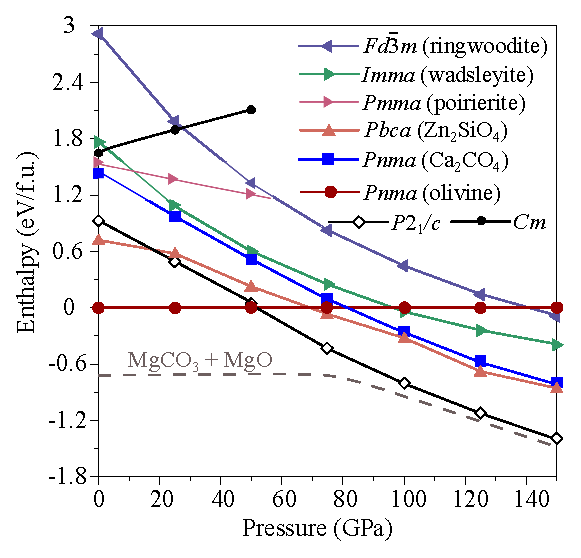
\includegraphics[width=0.6\textwidth]{E-P_mg2co4} \centering
	\caption{Enthalpy-pressure dependencies of Mg$_2$CO$_4$ structures. Isostructural compounds are indicated in brackets.
} \label{E-P}
\end{figure} 


Revealed Mg$_2$CO$_4$-$Pnma$ is isostructural to the mineral forsterite (Figure \ref{str}a,b).
Atoms in both positions Mg1 and Mg2 are 6-coordinated, with the octahedral coordination polyhedron (Figure \ref{str}c). 
Mg$_2$CO$_4$-$P2_1/c$ is isostructural to $\beta$-Ca$_2$SiO$_4$ (larnite) and can be considered as the monoclinic analogue of Ca$_2$CO$_4$-$Pnma$.
In crystal structure of Mg$_2$CO$_4$-$P2_1/c$, there are two non-equivalent Mg sites.
There is some ambiguity in determination of cooridnation numbers of Mg, due to the smooth variation of the bonds lengths.
In the first site Mg(1) is bonded to six oxygen atoms, arranged in highly deformed trigonal prism  (Figure \ref{str}d).
Lengths of the six Mg--O bonds within coordination polyhedron vary in the range 1.832--2.073 \AA, while the seventh oxygen atoms is distant on 2.382 \AA.
In the second site, Mg(2) is bonded to eight oxygen atoms, forming relatively regular square antiprism.
Lengths of these eight Mg--O bonds vary in the range of 1.887--2.126 \AA, while the neinth Mg--O bond is sufficiently longer, being equal to 2.688 \AA.
In Mg$_2$CO$_4$-$Pnma$ structure, oxygen atoms in the first coordination sphere is distant on 1,815--1.888 \AA\ for Mg(1) site and on 1.781--1.95 \AA\ --- for (Mg2) site.
All the presented bond lengths corresond to the pressure of 100 GPa.
In both $Pnma$ and $P2_1/c$ crystal structures, coordination polyhedrons around Mg atoms share both vertices and edges with [CO$_4$] tetrahedrons (Figure \ref{str}c,d).
%Thus, transition from Mg$_2$CO$_4$-$Pnma$ to Mg$_2$CO$_4$-$P2_1/c$ is accompanied by the increase of coordination number from six to eight and six.
Transition from Mg$_2$CO$_4$-$Pnma$ to Mg$_2$CO$_4$-$P2_1/c$ is accompanied by the sufficient decrease of the volume equal to 5.7 \% (Figure \ref{V-P}).

\begin{figure}[H]
	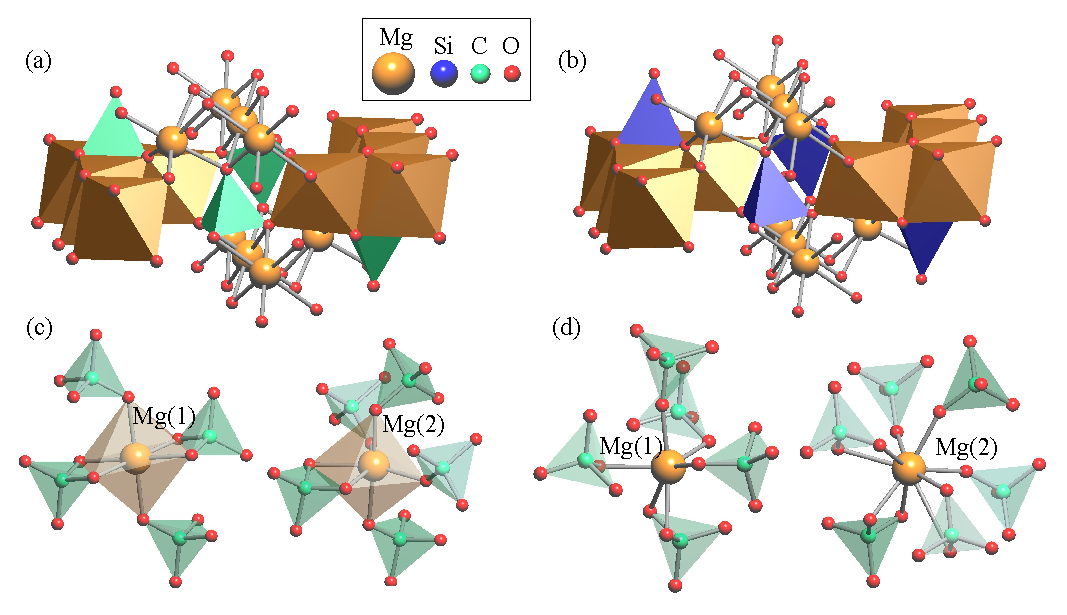
\includegraphics[width=\textwidth]{mg2co4_str} \centering
	\caption{Comparison of crystal structures of Mg$_2$CO$_4$-$Pnma$ (a) and Mg$_2$SiO$_4$-$Pnma$ (b) in projection on the (010) plane, coordination environment around Mg(1) and Mg(2) sites in crystals structures Mg$_2$CO$_4$-$Pnma$ (c) and Mg$_2$CO$_4$-$P2_1/c$ (d).} 	\label{str}
\end{figure}

Structural data for the Mg$_2$CO$_4$-$Pnma$ and Mg$_2$CO$_4$-$P2_1/c$ are given in the Table \ref{t:str}.
Both structures are dynamically stable in the investigated pressure range 0-140 GPa, and there are no imaginary frequencies in their phonon dispersion curves (Figure \ref{phon_mg2co4_main}, \ref{phon_mg2co4_supp}). 
The dynamical stability of the found Mg$_2$CO$_4$ structures at ambient pressure assume the possibility for their extraction from the chamber of the diamond anvill cell (DAC) after the high pressure synthesis and the further investgation with the technique of transmission electron microscopy.
In the {\it Supporting information}, we have also shown phonon dispersion curves of MgCO$_3$ and MgO (Figure \ref{phon_mgco3}) used for the construction of $P$--$T$ phase diagram.

\begin{table}[h] \centering
	\caption{Structural data of predicted Mg$_2$CO$_4$ phases at 0 K.} \vspace{2mm} \label{t:str}
	\begin{tabular}{l*{9}{l}}
		\hline \hline
		\multirow{2}*{$P$ (GPa)}	&	\multirow{2}*{Space group}	& \multicolumn{3}{c}{\multirow{2}*{Lattice parameters (\AA, deg)}}	&	\multirow{2}*{Atom}	&	\multicolumn{3}{c}{Coordinates} \\ 
		\cline{7-9}
		&&&&&&  x	&	y	&	z \\ 
		\hline 
		50 			&	 $Pnma\ (\#62)$ 				&	$a=8.926$ & $b=5.565$ & $c=4.221$		& 	Mg1					&	0.000	&	0.000	&	0.500 \\
		&&$\alpha$ = 90.0&$\beta$ = 90.0&$\gamma$ = 90.0&Mg2&0.721&0.250&0.531\\
		&&&&&C1&-0.097&0.250&0.087\\
		&&&&&O1&-0.091&0.250&0.770\\
		&&&&&O2&0.548&0.250&0.284\\
		&&&&&O3&0.169&0.552&0.786\\
		\hline
		100 			&	 $P2_1/c\ (\#14)$ 				&	$a=4.408$ & $b=5.383$ & $c=8.345$			& 	Mg1&0.702&0.360&0.425\\
		&&$\alpha$ = 90.0&$\beta$ = 117.65&$\gamma$ = 90.0& Mg2					&	-0.022	&	0.000	&	0.693 \\

		&&&&&C1&0.355&0.282&0.082\\
		&&&&&O1&0.146&0.334&0.638\\
		&&&&&O2&0.681&0.245&0.197\\
		&&&&&O3&0.272&0.168&-0.080\\	
		&&&&&O4&0.295&0.520&0.064\\	
		\hline \hline
	\end{tabular}
\end{table}


\begin{figure}[H]
	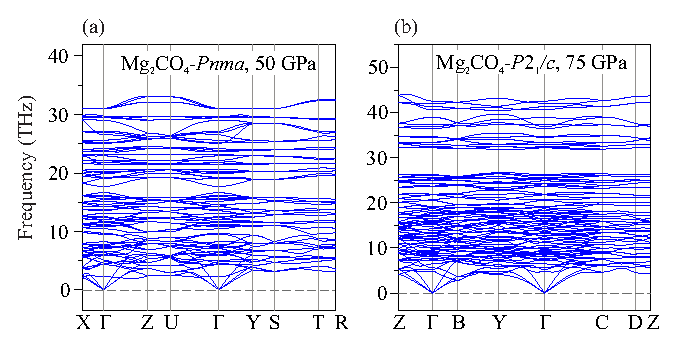
\includegraphics[width=\textwidth]{phon_mg} \centering
	\caption{Phonon dispersion curves of Mg$_2$CO$_4$-$Pnma$ (a-c) and Mg$_2$CO$_4$-$P2_1/c$ (d-f) at various pressures and 0 K.
	} 	\label{phon_mg2co4_main}
\end{figure}



There is no analogy of the found transition from Mg$_2$CO$_4$-$Pnma$ to Mg$_2$CO$_4$-$P2_1/c$ in the Mg$_2$SiO$_4$ system.
However, there is one in Ca$_2$SiO$_4$ system, where transformation of Mg$_2$CO$_4$-$Pnma$ into Mg$_2$CO$_4$-$P2_1/c$ corresponds to the transforamtion of $\gamma$-Ca$_2$SiO$_4$ into $\beta$-Ca$_2$SiO$_4$, which is alsi realized on compression \cite{belmonte2017}.
Heating of $\beta$-Ca$_2$SiO$_4$ produces the phase $\alpha_H'$-Ca$_2$SiO$_4$ and similar transition can be suggested for Mg$_2$CO$_4$.
In this case, heating of Mg$_2$CO$_4$-$P2_1/c$ will produce the new hypothetical phase Mg$_2$CO$_4$-$Pnma$-II similar to $\alpha_H'$-Ca$_2$SiO$_4$.
The performed calculations of phonon dispersion curves of Mg$_2$CO$_4$-$Pnma$-II, constructed based on the structure of $\alpha_H'$-Ca$_2$SiO$_4$ by corresponding atomic replacements, have shown the dynamical instability of this phase (Figure \ref{phon_PnmaII}).
However, the stabilization of the structure by the factors, which are not considered within QHA can not be excluded.




\subsubsection*{P--T phase diagram}

The performed enthalpy calculations of the Mg$_2$CO$_4$, MgO, and MgCO$_3$ structures have shown, that both Mg$_2$CO$_4$-$Pnma$ and Mg$_2$CO$_4$-$P2_1/c$ lie above the energetic convex hull, i.e. they are unstable and decompose to the mixture (MgO+MgCO$_3$) at 0 K (Figure \ref{conv_hull}). 

However, performed calculations of the Gibbs free energies in the temperature range of 0--3000 K have shown that above some temperature  Mg$_2$CO$_4$ became more energetically favorable than the (MgO+MgCO$_3$) mixture (Figure \ref{gibbs}).
At 20 GPa, this temperature is 2420 K, which is nearly equal to the melting temperature of  magnesite (MgCO$_3$-$R\bar{3}c$) \cite{solopova2015} (Figure \ref{phdia}).
With increasing the pressure the temperature of transition decreases, and at 140 GPa Mg$_2$CO$_4$-$P$2$_1$/$c$ became more favourable than the mixture of (MgO+MgCO$_3$) at temperatures higher than 1085 K.
Thus, in the pressure range of 50--140 GPa, Mg$_2$CO$_4$ can be synthesised at temperatures 250--1100 K higher than the corresponding temperatures of MgCO$_3$ melting (Figure \ref{phdia}). 
It suggests the possibility for the formation of Mg-orthocarbonate in most part of the Earth's lower mantle, at pressures higher than 50 GPa.

\begin{figure}[H]
	\centering
	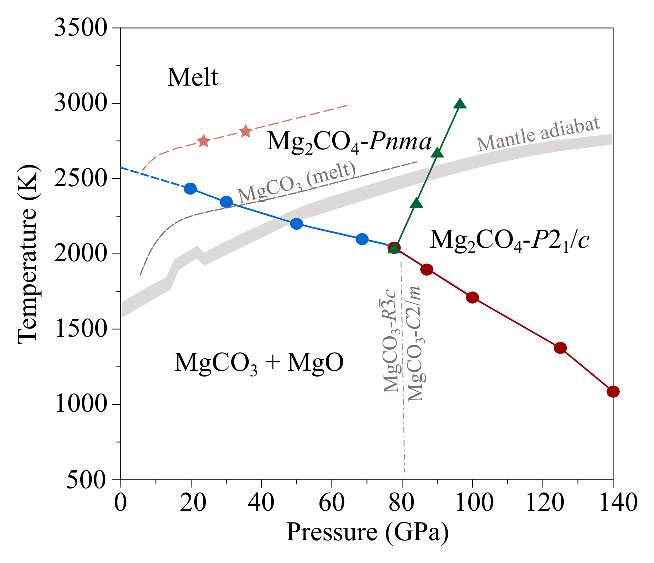
\includegraphics[width=0.6\textwidth]{phdia_mg2co4}
	\caption{$P$--$T$ phase diagram of Mg$_2$CO$_4$. The asterisks represent calculated melting temperatures;  the grey dash-dotted line --- calculated phase transition boundary of MgCO$_3$; the grey dashed line --- melting curve of MgCO$_3$ as reported by Solopova et al. \cite{solopova2015}; grey solid line --- mantle adiabat according to  Katsura \cite{katsura2010}.} 
\label{phdia}
\end{figure}


\subsubsection*{Raman spectra}

As Raman techniqe are now actively used for the identification of $sp^3$ bonded carbonates and orthocarbonates in high-pressure DAC experiments \cite{lobanov2017, binck2020_mgco3}, we have calculted Raman spectra for the Mg$_2$CO$_4$-$Pnma$ phase.

The unit cells of Mg$_2$CO$_4$-$Pnma$ contain 28 atoms, i.e. there are 84 phonon modes. 
According to a group theoretical analysis, 36 Raman active modes are expected for Mg$_2$CO$_4$-$Pnma$: $\Gamma = 11A_g + 7B_{1g} + 11B_{2g} + 7B_{3g}$. 
The most intense mode (B$_{2g}$) corresponds to the bending and stretching vibrations in the [CO$_4$] tetrahedral groups and appears at 1025 cm$^{-1}$. 
The second (A$_g$) and third (B$_{1g}$) most intense modes appear at 1089 and 1106 cm$^{-1}$, correspondingly (Figure \ref{displ}). The calculated Raman spectra at 60 GPa is shown in Figure \ref{raman}.

\begin{figure}[H]
	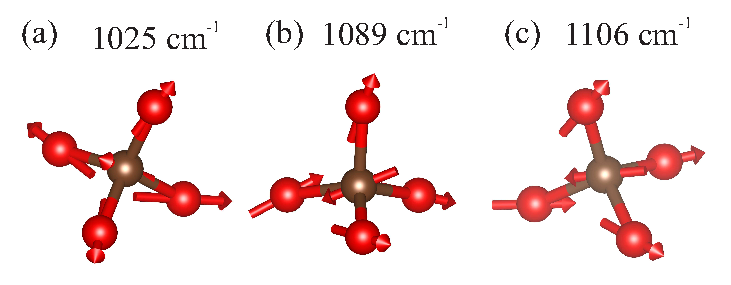
\includegraphics[width=0.5\textwidth]{dis_pat} \centering
	\caption{Displacement patterns in Raman modes of Mg$_2$CO$_4$-$Pnma$ at 60 GPa. Arrows indicate the displacement of the atoms during the specific vibration.} \label{displ}
\end{figure}

\begin{figure}[H]
	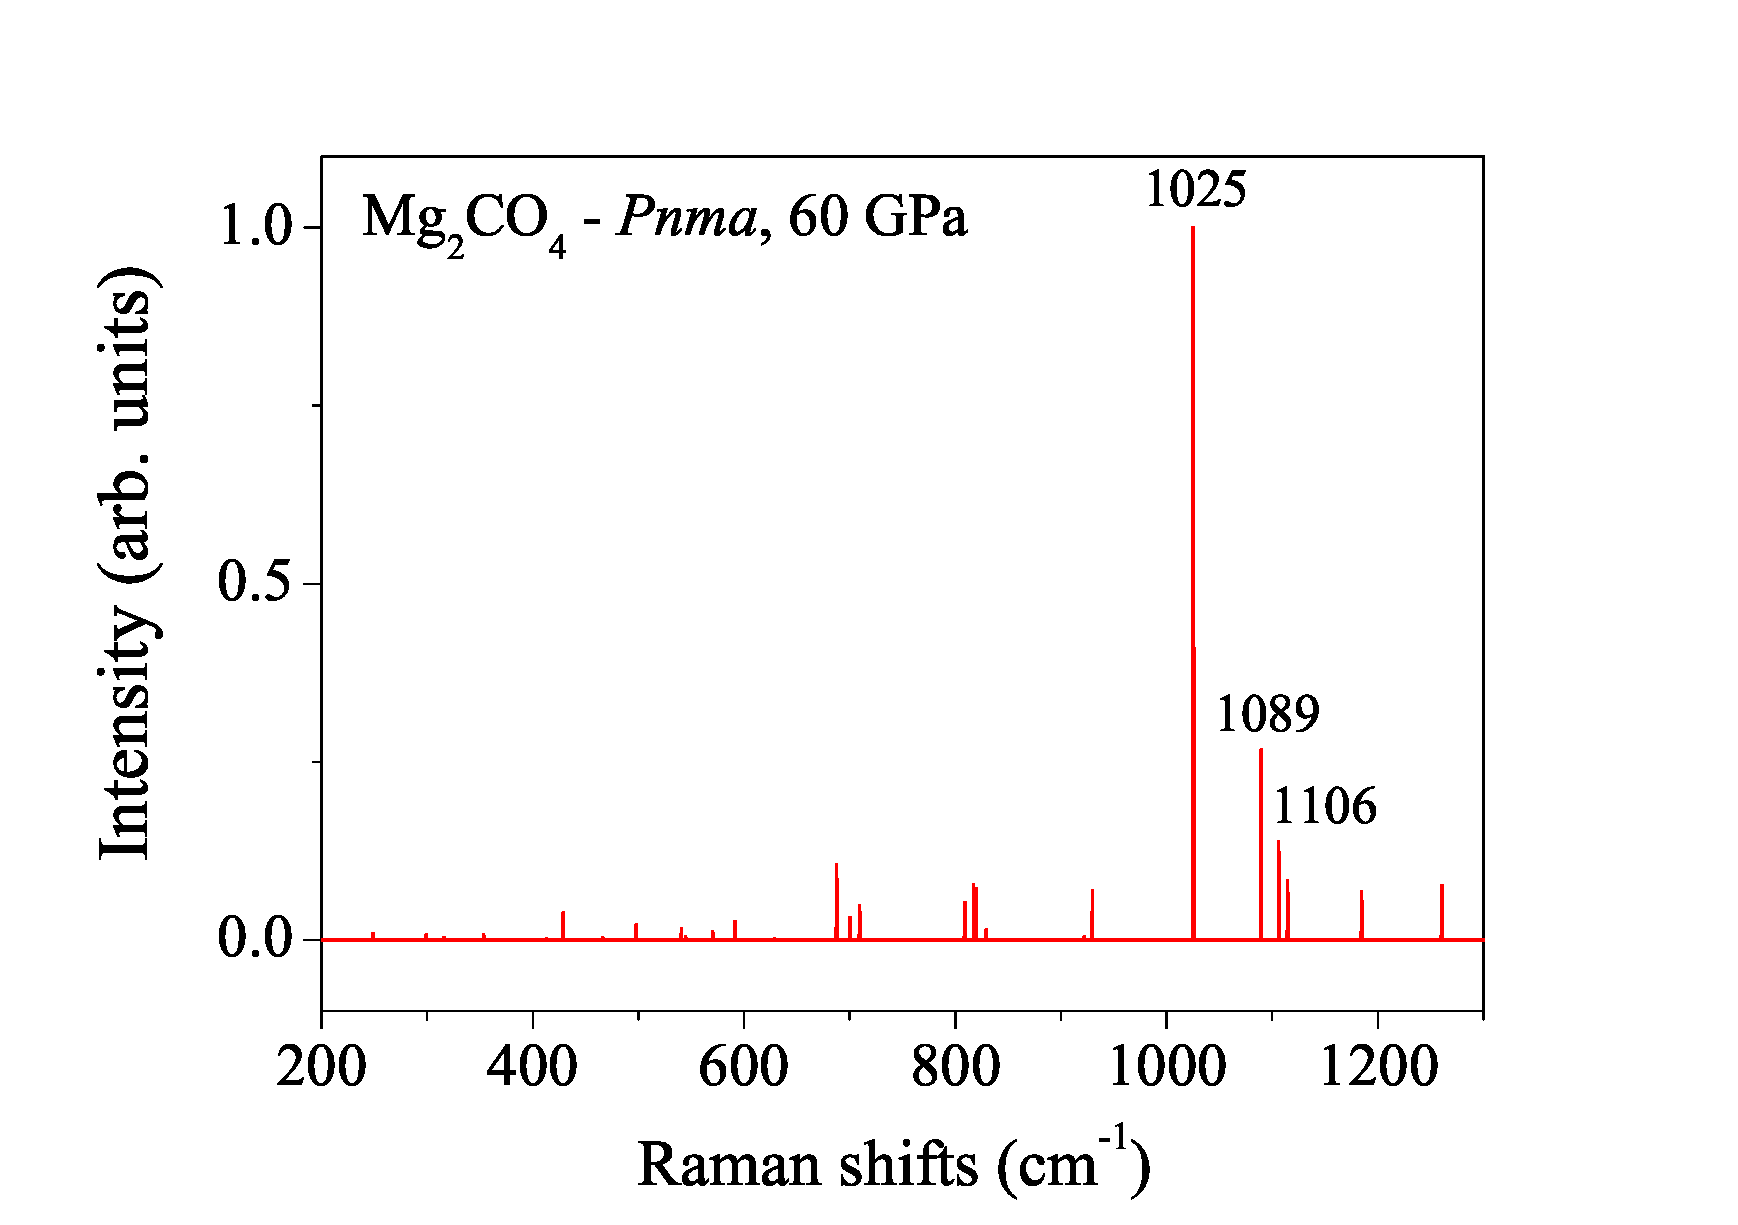
\includegraphics[width=0.7\textwidth]{raman_mg2co4} \centering
	\caption{DFT-calculated Raman spectra of Mg$_2$CO$_4$-$Pnma$ at 60 GPa.} \label{raman}
\end{figure}


\subsubsection*{Analysis of electronic denisty distribution}

In both found structures, $Pnma$ and $P2_1/c$, four C--O bonds within [CO$_4$] tetrahedron are of nearly the same length.
At 100 GPa, these bond distances vary in the range 1.32--1.37 \AA\ in both structures. 
The similar values of bond lengths assume the covalent nature for all four bonds.
The performed analysis of electron density distribution confirms this assumption.
The isosurface of the electron desity difference clearly shows the accumulation of charge halfway along each of the four C—O bond (Figure \ref{diff}).


\begin{figure}[H]
	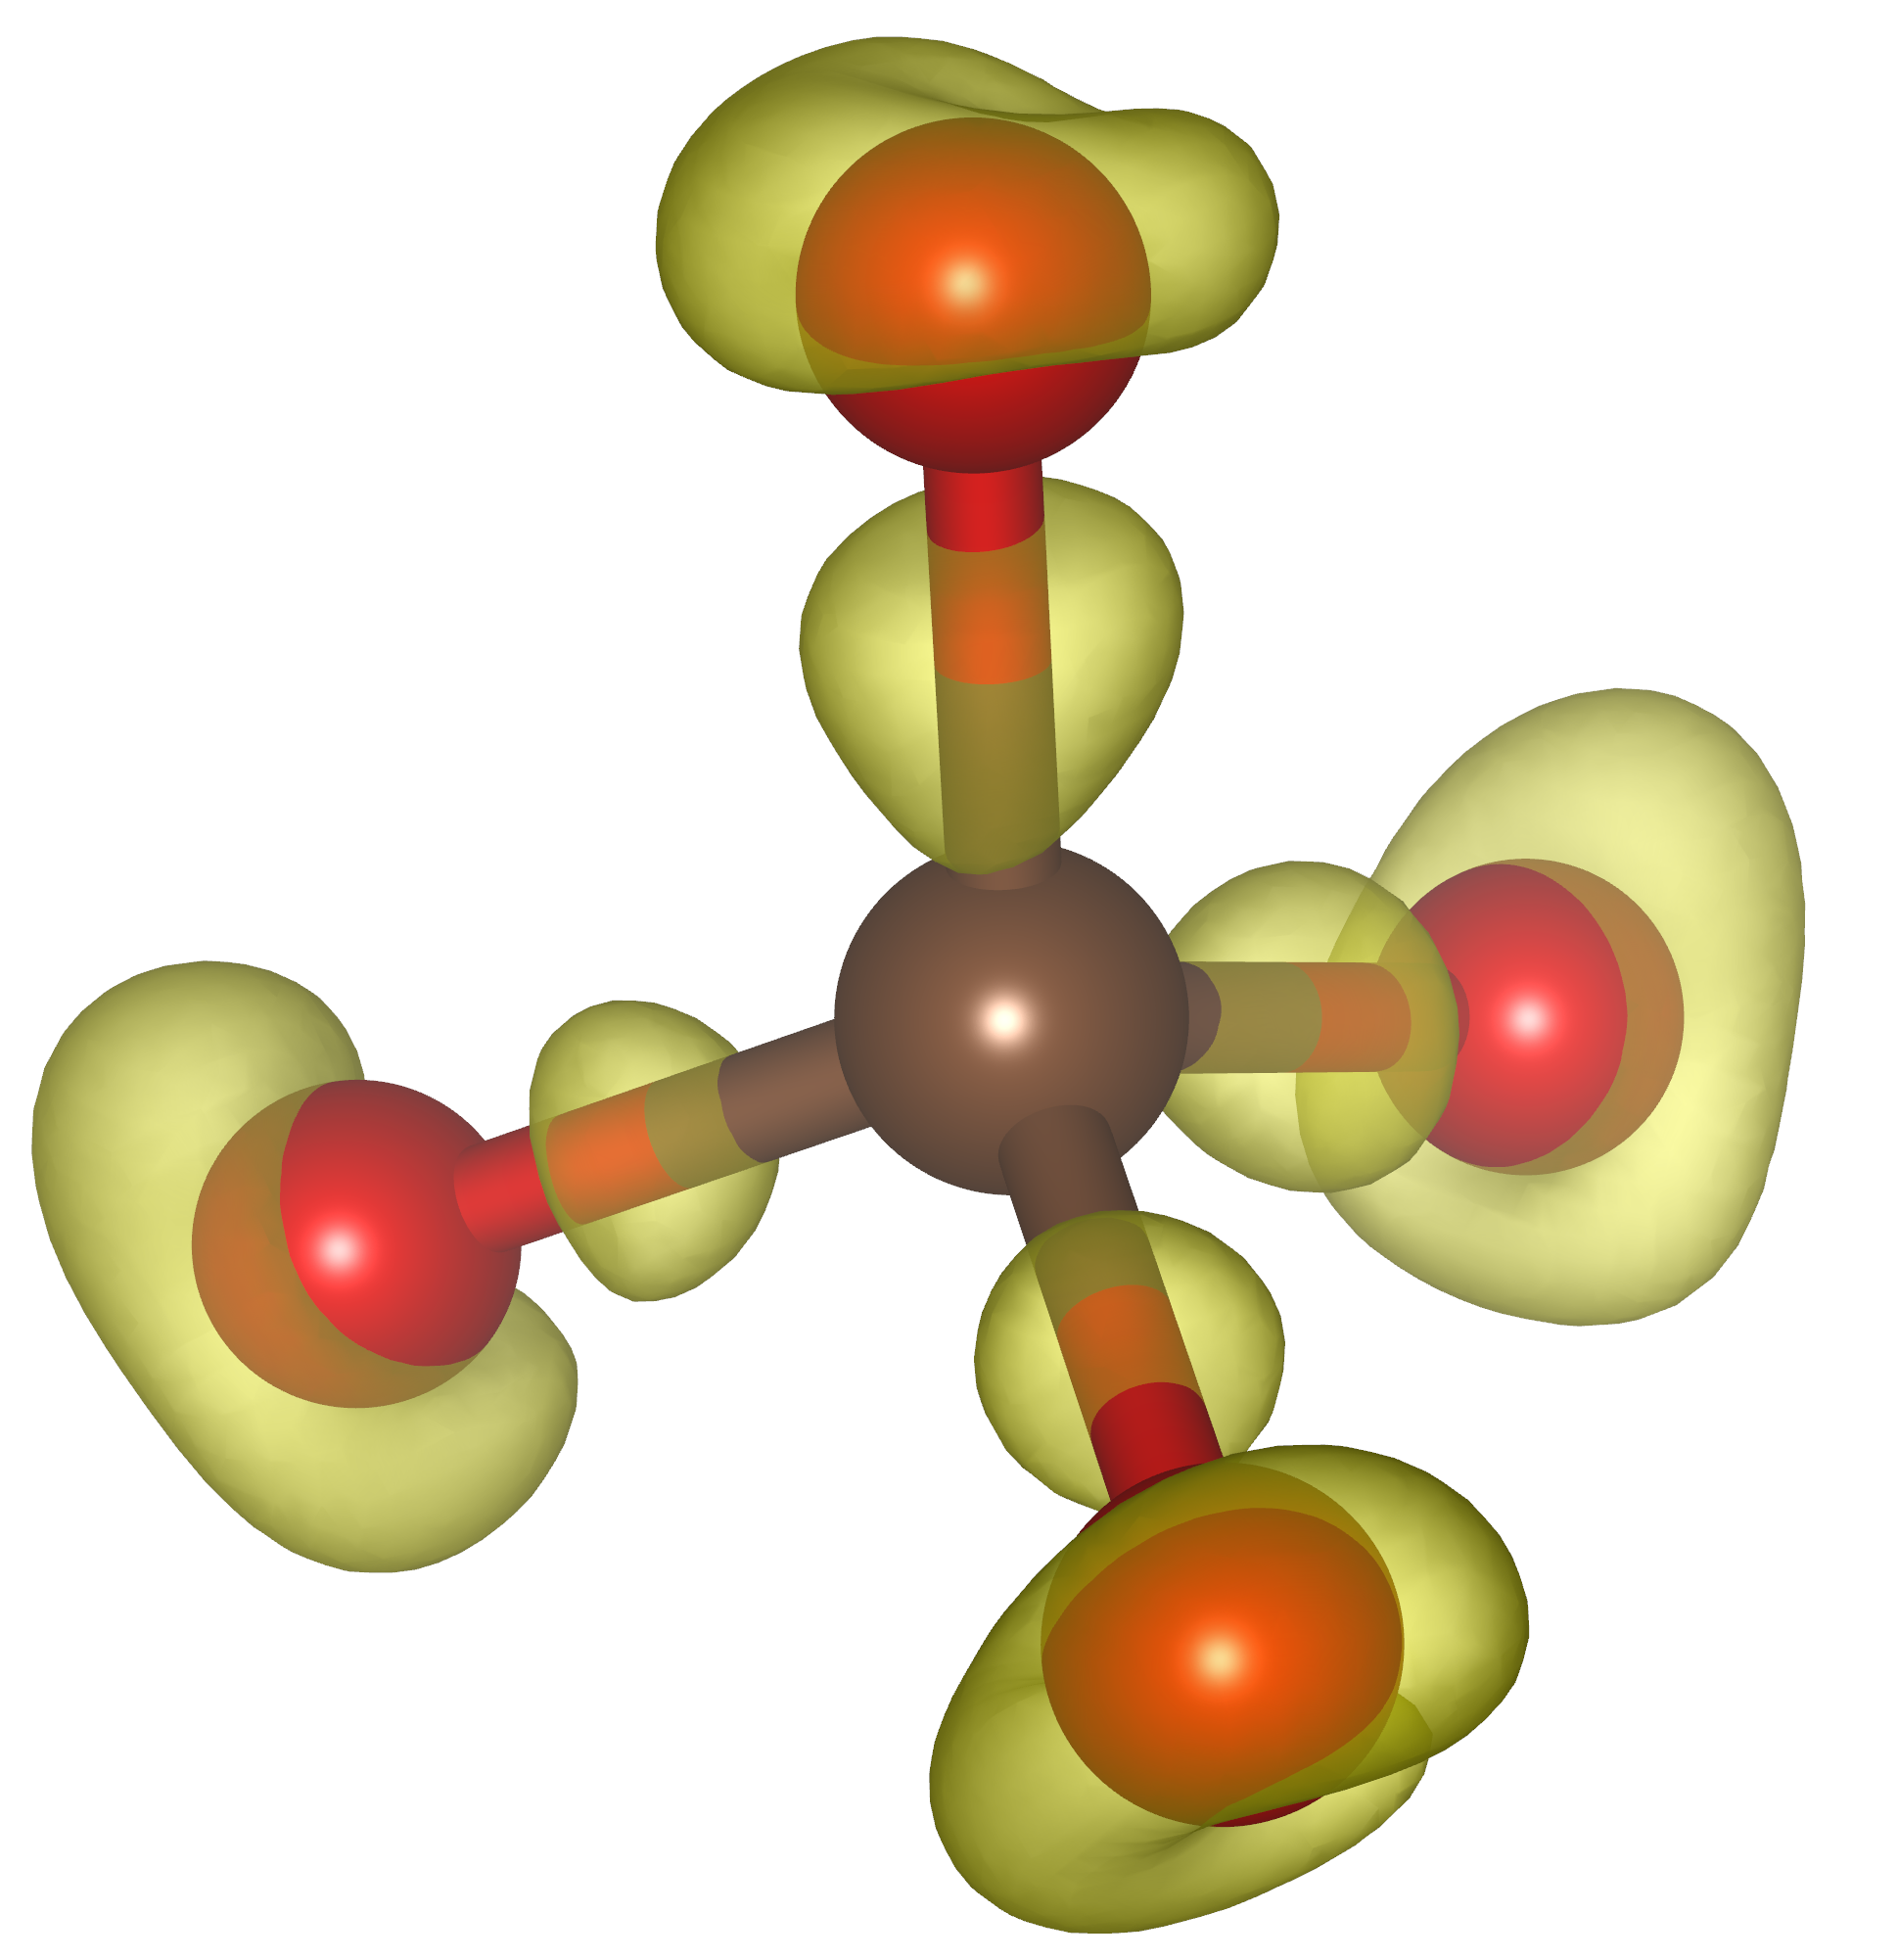
\includegraphics[width=0.5\textwidth]{dens_diff.png} \centering
	\caption{Isosurface of the electron density difference in Mg$_2$CO$_4$-$Pnma$ structure. The isosurface shows those regions in which the electron density is larger than that obtained by overlapping electron densities of non-interacting atoms.} \label{diff}
%! У Ланиэля еще указывается The isosurface is plotted fora value of 0.2 e A3
%! {У нас в isosurface я ставил значение 0.042, подумал не мало ли это и не стал указывать. У Винклера значение 0.2}
%! Нам тоже нужно указать для какого сечения мы строим распрпделение электронной плотности.
\end{figure}

The isostructural character of Mg$_2$CO$_4$-$Pnma$ and Mg$_2$SiO$_4$-$Pnma$ gives a rare possibility for performing the comparison of electron density distribution in the structures of orthocarbonate and orthosilicate.

At 0 GPa, the Si--O bond is longer than C--O bond on 15-19 \%.
According to the classical rule of isomorphism, suggested by Goldschmidt, the isomorphism in the wide range of compositions require the difference of atomic radii on no more than 15 \%.
The obtained value is on the border of this limit and from the first glance the possibility of the (Si,C) isomorphism at high temperatures can not be excluded.
However, it is not the case, as isomorhism requires similar nature of the bonds around atoms substituting each other.
The obtained Bader charge of C$^{4+}$ is predictably lower than that of Si$^{4+}$, 1.914 against 3.109. 
This indicates on the more covalent character of C--O bond in comparison with the Si--O bond.
Bader charges of the other atoms are summarised in Table \ref{t:bader}.

\begin{table}[h] \centering
	\caption{Comparison of Bader charges on atoms in Mg$_2$SiO$_4$-$Pnma$ and Mg$_2$CO$_4$-$Pnma$ structures at 0 GPa (in unit of e).} \vspace{2mm} \label{t:bader}
	\begin{tabular}{l l l l l l l }
        &       Mg1     &       Mg2     &       C/Si    &       O1      &       O2      &       O3      \\
		\hline
Mg$_2$SiO$_4$ &       1.731   &       1.745   &       3.109   &       -1.645  &       -1.657  &       -1.641  \\
Mg$_2$CO$_4$  &       1.724   &       1.745   &       1.914   &       -1.412  &       -1.340  &       -1.315  \\
		\hline 


	\end{tabular}
\end{table}


\subsubsection*{Melting temperature and seismic properties}
To compare the melting temerature of Mg-carboante and Mg-orhtocarboantes, we have estimated melting temperatures of Mg-orthocarbonate.
The obtained values of the Mg$_2$CO$_4$-$Pnma$ melting temperatures at 23.7 GPa, 35.5 GPa and 52.2 GPa equal to 2661 K, 2819 K, and 3109 K, respectively (Figure \ref{Zcurve}).
These values are 14-22 \% higher than the experimentally measured melting temperatures of magnesite and comparable with solidi of silicate rocks under lower mantle P--T conditions \cite{litasov2018_review}.
As can be seen from Figure \ref{phdia} the difference in melting temperatures promptly increases with pressure, reaching 500 K at nearly 40 GPa.



To assess the effect of orthocarbonate formation on the seismic properties of carbonate, we have also calculated the elastic stiffness tensor and compressional/shear sound velocities ($V_p$/$V_s$) for Mg-carbonate and Mg-orthocarbonate.
We have not aimed the investigation of trends for the changes of elastic properties on compression or their description during $Pnma$ $\to$ $P2_1/c$ transition, but only the rough comparison of carbonate and orthocarbonate properties.
By this reason, calculations have been performed only at 50 GPa and 0 K for Mg$_2$CO$_4$-$Pnma$ and magnesite structures.

The obtained elastic properties of Mg$_2$CO$_4$-$Pnma$ and magnesite are summarized in Table \ref{elastic_const} and Table \ref{moduli}.
Obtained values of $C_{ij}$, $B$, $G$, $V_p$, and $V_s$ for magnesite are in good agreement with the previous results of theoretical calculations \cite{li2020_mgco3}.
According to our results, the density and both bulk and shear moduli of Mg$_2$CO$_4$-$Pnma$ are higher than that of magnesite by 4-5 \%.
Orthocarbonate is similar to carbonate in sense of seismic velocities $V_p$ and $V_s$, but orthocarbonate is more anisotropic, owning higher universal anisotropy ($A^U$).
The value of $A^U$ for Mg$_2$CO$_4$-$Pnma$ is 0.4772, while that for magnesite is 0.2838.


%%%%%%%%%%%%%%%%%%%%%%%
\section*{Acknowledgments}
%%%%%%%%%%%%%%%%%%%%%%%
This study was funded by the RFBR under research projects \#20-03-00774 and \#20-35-90043.
Crystal structure prediction and calculation of $P$--$T$ phase diagram were performed within the project \#20-03-00774, while calculations of melting curve --- within the project \#20-35-90043.
Calculations of elastic properties were supported by a state-assigned project of the IGM SB RAS. 

The computations were performed using resources provided by the Novosibirsk State University Supercomputer Center.


\bibliographystyle{CGD}
\bibliography{refs_mg2co4}

\end{document}


